% Smart Dustbin SRS
% Compile twice with pdfLaTeX to update the contents.
% Diagrams are editable TikZ code. No external image files are needed.
\documentclass[11pt,a4paper]{article}
\usepackage[T1]{fontenc}
\usepackage[utf8]{inputenc}
\usepackage{lmodern}
\usepackage[margin=20mm,headheight=14pt]{geometry}
\usepackage{microtype}
\usepackage{array,tabularx,longtable,booktabs}
\usepackage{amsmath}
\usepackage{tikz}
\usetikzlibrary{arrows.meta,positioning,shapes.geometric,calc}
\usepackage{fancyhdr}
\usepackage{titlesec}
\usepackage[hidelinks]{hyperref}
\hypersetup{pdftitle={Smart Dustbin System Requirements Specification},pdfauthor={Group 06}}
\setlength{\parindent}{0pt}
\setlength{\parskip}{7pt}
\setlength{\emergencystretch}{3em}
\renewcommand{\arraystretch}{1.14}
\setlength{\tabcolsep}{5pt}
\pagestyle{fancy}
\fancyhf{}
\fancyhead[L]{\footnotesize Smart Dustbin}
\fancyhead[R]{\footnotesize System Requirements Specification}
\fancyfoot[C]{\thepage}
\renewcommand{\headrulewidth}{0pt}
\titleformat{\section}{\large\bfseries}{}{0pt}{}
\titleformat{\subsection}{\normalsize\bfseries}{}{0pt}{}
\titlespacing*{\section}{0pt}{0pt}{12pt}
\titlespacing*{\subsection}{0pt}{10pt}{5pt}
\newcolumntype{Y}{>{\raggedright\arraybackslash}X}
\tikzset{block/.style={draw,rounded corners=2pt,align=center,font=\small,text width=3.5cm,minimum height=1.15cm,inner sep=5pt,execute at begin node={\setlength{\parskip}{0pt}}},arrow/.style={-{Latex[length=2mm]},thin},wire/.style={thin}}
\newcommand{\reportsection}[1]{\section*{#1}\addcontentsline{toc}{section}{#1}}
\newcommand{\reportsubsection}[1]{\subsection*{#1}\addcontentsline{toc}{subsection}{#1}}
\begin{document}
\begin{titlepage}
\centering
\vspace*{12mm}
{\Large\bfseries Bangladesh University of Professionals\par}
\vspace{5mm}
Faculty of Science and Technology\par
Department of Computer Science and Engineering\par
\vspace{22mm}
{\LARGE\bfseries System Requirements Specification\par}
\vspace{8mm}
{\Large\bfseries ESP32 Based Smart Waste Bin\par}
\vspace{3mm}
Real Time Monitoring and Collector Dashboard\par
\vspace{18mm}
Computer Interfacing Laboratory\par
Course Code: CSE 4102\par
Section: B\par
Group: 06\par
\vspace{12mm}
\textbf{Submitted by}\par
\vspace{4mm}
\begin{tabular}{@{}ll@{}}
Sheikh Sifat Rahman & 23524242108 \\
Sajid Al Adeeb & 23524242030 \\
Abdullah Towhid & 23524242054 \\
Taqi Tahmid & 23524242110
\end{tabular}
\vfill
Date of Submission: 5 October 2026\par
\vspace*{12mm}
\end{titlepage}
\setcounter{page}{2}
\tableofcontents

\clearpage
\reportsection{1 Introduction}
\reportsubsection{1.1 Background and motivation}
A caretaker usually finds out whether a dustbin is full by walking up to it and looking inside. If the bin is nearly empty, the visit may not lead to any action. If it fills soon after the visit, waste may remain there until the next inspection. As the number of bins grows, keeping track of them becomes harder.\par

There is also a smaller problem at the bin itself. A person may need to touch the lid before throwing waste away. An automatic lid can make this easier, but it does not tell a collector when the bin needs to be emptied. This project brings these two needs together.\par

The Smart Dustbin will open when its IR sensor detects a hand. A separate ultrasonic sensor will measure the distance to the waste. The readings will then appear on a local dashboard, where a collector can see which bin needs attention and when it was last emptied.\par

\reportsubsection{1.2 Objectives}
1. To open and close the lid without requiring the user to touch it.\par

2. To measure fill level using one ultrasonic sensor and show it as a percentage.\par

3. To read temperature and humidity and show useful information on an LCD.\par

4. To let collectors view bin locations, readings, opening counts, and collection history.\par

5. To estimate the next collection time and demonstrate the complete system on local Wi-Fi.\par

\reportsubsection{1.3 Scope}
The project includes one physical bin, simulated bins, an ESP32, a local server, a database, and a browser dashboard. Both the hardware and the dashboard will use the same Wi-Fi network. Bin locations will be written as text addresses. The project does not include waste sorting, weighing, GPS maps, vehicle routes, or cloud access.\par

\reportsubsection{1.4 Intended users}
People using the bin will interact with its automatic lid. Collectors will use the dashboard to plan visits and review collections. The project team will set up and test the system. Course evaluators will review how the hardware and software work together.\par


\clearpage
\reportsection{2 Existing System and Requirements Discovery}
\reportsubsection{2.1 What existing systems offer}
A normal dustbin is simple to use, but its condition is only known when someone checks it. Some small electronic projects improve this by adding an automatic lid. Arduino Education, for example, describes a trash can that uses an ultrasonic sensor and a servo to open when a person approaches [R4].\par

Arduino Cloud also describes a smart trash can with automatic opening and an option to open it through the cloud [R5]. These examples show how touchless access can work. Their cited descriptions focus on lid control rather than the collection records and local collector view needed for this project.\par

\textbf{Table 2.1 Comparison of existing approaches}\par
{\small
\begin{longtable}{@{}>{\raggedright\arraybackslash}p{3.536cm}>{\raggedright\arraybackslash}p{5.350cm}>{\raggedright\arraybackslash}p{6.334cm}@{}}
\toprule
\textbf{System} & \textbf{What it provides} & \textbf{What this project adds} \\ \midrule
\endhead
Normal dustbin & A place to store waste; checked by hand. & Fill readings and a shared view of bin condition. \\[3pt]
Arduino Education example [R4] & Proximity sensing and servo lid control. & Separate fill sensing, environment readings, and collection tracking. \\[3pt]
Arduino Cloud example [R5] & Automatic opening and cloud control. & A collector dashboard designed to work locally without internet. \\[3pt]
\bottomrule
\end{longtable}
}
\reportsubsection{2.2 How the requirements were found}
The starting point was the project proposal [R1]. The collector dashboard plan [R2] then explained how several bins would appear on one screen and how the readings would be stored. These documents describe the monitoring features and hardware needed for the prototype.\par

\reportsubsection{2.3 The proposed solution}
The updated design uses an IR obstacle sensor to detect a hand and one ultrasonic sensor to measure fill distance. The ESP32 handles the lid and sends readings through Wi-Fi. The local server turns those readings into fill information, collection records, and an estimate of the next collection time.\par

The dashboard uses Node.js, Express, SQLite, and plain JavaScript. A manual collection button is also included, so the collector can record an emptying that automatic detection does not recognize.\par


\clearpage
\reportsection{3 User and System Requirements}
\reportsubsection{3.1 User requirements}
A person using the bin should not need to understand the electronics. A collector should be able to open the dashboard and quickly see what needs attention. The following requirements describe those needs.\par

\textbf{UR01.} The system shall open the lid when a hand is detected near the IR obstacle sensor.\par

\textbf{UR02.} The system shall close the lid after the hand has been removed for the configured time.\par

\textbf{UR03.} The system shall let a collector view all registered bins and open a separate page for each bin.\par

\textbf{UR04.} The system shall show a bin's address, fill level, last collection time, and number of lid openings since collection.\par

\textbf{UR05.} The system shall show temperature, humidity, connection status, and the time of the latest reading.\par

\textbf{UR06.} The system shall show an estimated next collection time, or explain why there is not enough data to calculate it.\par

\textbf{UR07.} The system shall let the collector mark a bin as collected after emptying it.\par

\textbf{UR08.} The system shall continue local lid operation when Wi-Fi is unavailable and distinguish physical bins from simulated bins.\par

\subsection*{What the numbers mean}
The usage count means lid openings, not items of waste. The collection time is a recorded event, not proof of a scheduled visit. The estimated next collection time is a guide based on recent fill changes. These meanings shall be clear on the dashboard.\par


\clearpage
\reportsubsection{3.2 Functional Requirements}
Functional requirements describe what happens as a person uses the bin and the collector checks its records. Each statement below describes one required behaviour [R7, R8].\par

\subsection*{At the physical bin}
\textbf{FR01.} The controller shall open the lid when the IR obstacle sensor detects a hand.\par
\textbf{FR02.} The controller shall keep the lid open while the IR sensor detects a hand.\par
\textbf{FR03.} The controller shall close the lid after the sensor has remained clear for the configured delay.\par
\textbf{FR04.} The controller shall reopen the lid if it detects a hand during closing.\par
\textbf{FR05.} The controller shall count each commanded opening cycle once.\par
\textbf{FR06.} The controller shall obtain fill distance from one ultrasonic sensor after the closed lid has settled.\par
\textbf{FR07.} The controller shall obtain temperature and humidity from the DHT11.\par
\textbf{FR08.} The controller shall represent unavailable sensor readings as null in transmitted data.\par
\textbf{FR09.} The controller shall send sensor readings and opening increments to the local server at the configured interval.\par
\textbf{FR10.} The controller shall retain unacknowledged opening increments for retry while it remains powered.\par
\textbf{FR11.} The LCD shall display temperature, humidity, Wi-Fi state, and the latest fill value received from the server.\par
\textbf{FR12.} The LCD shall identify a stored fill value as old when it cannot be refreshed.\par

\clearpage
\section*{3.2 Functional Requirements Continued}
\subsection*{At the server and dashboard}
The server checks each incoming reading before updating the bin record. The collector can then review the results or record an emptying that was not detected automatically.\par

\textbf{FR13.} The server shall validate incoming readings against registered bin IDs and permitted field types and ranges.\par
\textbf{FR14.} The server shall store accepted readings with their receipt time.\par
\textbf{FR15.} The server shall process each submission ID only once.\par
\textbf{FR16.} The server shall calculate fill percentage from valid distance readings using the selected bin's calibration.\par
\textbf{FR17.} The server shall record a collection when stable fill changes from the configured high threshold to the configured low threshold.\par
\textbf{FR18.} The dashboard shall request confirmation before recording a manual collection.\par
\textbf{FR19.} The server shall reset the opening count after a recorded collection.\par
\textbf{FR20.} The server shall estimate the next collection time from sufficient recent stable readings with a positive fill rate.\par
\textbf{FR21.} The overview shall show each bin's location, fill level, temperature, humidity, connection status, and last collection time.\par
\textbf{FR22.} Each bin detail page shall show its readings, opening count, fill chart, collection history, and collection estimate or reason for its absence.\par
\textbf{FR23.} The dashboard shall identify missing values and last known readings when current data is unavailable.\par
\textbf{FR24.} The dashboard shall mark a bin offline after 30 seconds without an accepted reading.\par
\textbf{FR25.} The demo shall submit simulated and manually entered raw readings through the same API used by the physical bin.\par
\textbf{FR26.} The dashboard shall label simulated bins separately from physical bins.\par

\clearpage

\reportsubsection{3.3 Non Functional Requirements}
The features explain what the system does; the following requirements explain how well it should work and the conditions it must support [R8]. These are proposed acceptance targets for the laboratory prototype, not measured results.\par

\textbf{Table 3.1 Quality requirements}\par
{\small
\begin{longtable}{@{}>{\raggedright\arraybackslash}p{3.620cm}>{\raggedright\arraybackslash}p{11.960cm}@{}}
\toprule
\textbf{ID and quality} & \textbf{Requirement} \\ \midrule
\endhead
NFR01 Accuracy & At each of five known fill heights, at least 9 of 10 settled readings shall be within 5 percentage points of the calibrated fill percentage. \\[5pt]
NFR02 Lid response & Lid movement shall begin within 1 second of a valid hand detection during normal powered operation. \\[5pt]
NFR03 Display response & An accepted reading shall appear on the dashboard within 15 seconds on a healthy local Wi-Fi network. \\[5pt]
NFR04 Reliability & The prototype shall complete a 30 minute demonstration without a controller reset or server crash. \\[5pt]
NFR05 Network tolerance & Local lid control shall remain operational throughout a 60 second Wi-Fi outage. \\[5pt]
NFR06 Power stability & The controller shall complete 20 consecutive lid cycles with Wi-Fi active without a brownout. \\[5pt]
NFR07 Data durability & All acknowledged readings and collection records shall remain available after a normal server restart. \\[5pt]
NFR08 Navigation & Any listed bin's detail page shall be reachable with one selection from the overview. \\[5pt]
NFR09 Readability & Every colour used to indicate bin status shall have an accompanying text label. \\[5pt]
NFR10 Local availability & All dashboard pages, fonts, and charts shall remain usable without internet access while the local server and Wi-Fi are available. \\[5pt]
NFR11 Maintainability & Bin calibration and collection thresholds shall be adjustable through configuration without changes to calculation logic. \\[5pt]
NFR12 Electrical compatibility & Every controller input shall remain within the selected board's specified input voltage limits during operation [R6]. \\[5pt]
\bottomrule
\end{longtable}
}

\clearpage

\reportsection{4 Hardware and Software Requirements}
\reportsubsection{4.1 Hardware requirements and budget}
Only one set of bin hardware is needed for the demonstration. The other bins will be simulated. Table 4.1 gives planning allowances in Bangladeshi taka. These are estimated budget amounts, not supplier quotations or confirmed purchase prices.\par

\textbf{Table 4.1 Hardware and planned costs}\par
{\small
\begin{longtable}{@{}>{\raggedright\arraybackslash}p{6.426cm}>{\raggedright\arraybackslash}p{6.918cm}>{\raggedright\arraybackslash}p{1.876cm}@{}}
\toprule
\textbf{Component and quantity} & \textbf{Purpose} & \textbf{BDT} \\ \midrule
\endhead
ESP32 board \(\times\)1 & Read sensors and connect through Wi-Fi & 650 \\[3pt]
HC-SR04 \(\times\)1 & Measure distance to waste & 120 \\[3pt]
IR obstacle sensor \(\times\)1 & Detect a hand near the lid & 80 \\[3pt]
SG90 servo \(\times\)1 & Open and close the lid & 180 \\[3pt]
DHT11 module \(\times\)1 & Read temperature and humidity & 150 \\[3pt]
16x2 LCD with I2C backpack \(\times\)1 & Show local information & 300 \\[3pt]
Breadboard \(\times\)1 & Hold the prototype circuit & 120 \\[3pt]
Jumper wire set \(\times\)1 & Connect the components & 100 \\[3pt]
Resistors and capacitor set & Voltage divider and power support & 70 \\[3pt]
Logic level shifter \(\times\)1 & Connect a 5 V I2C LCD safely & 80 \\[3pt]
Regulated 5 V supply \(\times\)1 & Provide adequate current & 300 \\[3pt]
USB cable \(\times\)1 & Program and power the board as suitable & 100 \\[3pt]
Bin, mounts, and linkage & Hold the components and move the lid & 400 \\[3pt]
Subtotal & One physical prototype & 2750 \\[3pt]
Extra allowance & 10\% for small additional parts & 275 \\[3pt]
Total planned budget & Excludes existing laptop and Wi-Fi device & 3025 \\[3pt]
\bottomrule
\end{longtable}
}
The LCD is assumed to have an I2C backpack. This must be checked before final wiring. The servo must also be tested with the selected lid. A heavy lid may need a different motor or a lighter mechanism.\par


\clearpage
\reportsubsection{4.2 Software Requirements}
The hardware needs firmware to read sensors and move the lid. The computer then needs a small server to store the readings and a browser page to show them. Using these three parts keeps the work easy to build and test in stages.\par

\textbf{Table 4.2 Software requirements}\par
{\small
\begin{longtable}{@{}>{\raggedright\arraybackslash}p{3.075cm}>{\raggedright\arraybackslash}p{5.842cm}>{\raggedright\arraybackslash}p{6.303cm}@{}}
\toprule
\textbf{Part} & \textbf{Software} & \textbf{Purpose} \\ \midrule
\endhead
Firmware & Arduino IDE, ESP32 board support, C/C++ & Build and upload the ESP32 program. \\[3pt]
Device communication & ESP32 Wi-Fi and HTTP client support & Send readings to the local server. \\[3pt]
Hardware libraries & ESP32 compatible servo, DHT, and I2C LCD libraries & Control the selected modules. Exact library versions will be fixed during implementation. \\[3pt]
Backend & Node.js and Express & Check data, calculate values, and serve the dashboard. \\[3pt]
Database & SQLite with better-sqlite3 proposed & Store bin details, readings, and collection events. \\[3pt]
Dashboard & HTML, CSS, and plain JavaScript & Show the collector interface in a browser. \\[3pt]
Charts & Chart.js bundled locally & Draw fill history without an internet download. \\[3pt]
Simulator & Node.js script & Send test readings using the real API. \\[3pt]
\bottomrule
\end{longtable}
}
\subsection*{Local network setup}
The ESP32, server computer, and dashboard device will join the same local network. The network must allow devices to reach each other. A tested hotspot can be used if a university network blocks this traffic. The selected ESP32 requires a compatible 2.4 GHz Wi-Fi network [R6].\par

The dashboard and its chart files shall be available on the local server without an internet connection. The server shall save collection records and display times in Asia/Dhaka.\par

\clearpage
\reportsection{5 System Design and Architecture}
\reportsubsection{5.1 Circuit Diagram}
The ESP32 connects the sensors, lid motor, and LCD. The IR sensor detects a hand, while one ultrasonic sensor measures the distance to the waste. Figure 5.1 shows the proposed connections.\par

\begin{center}
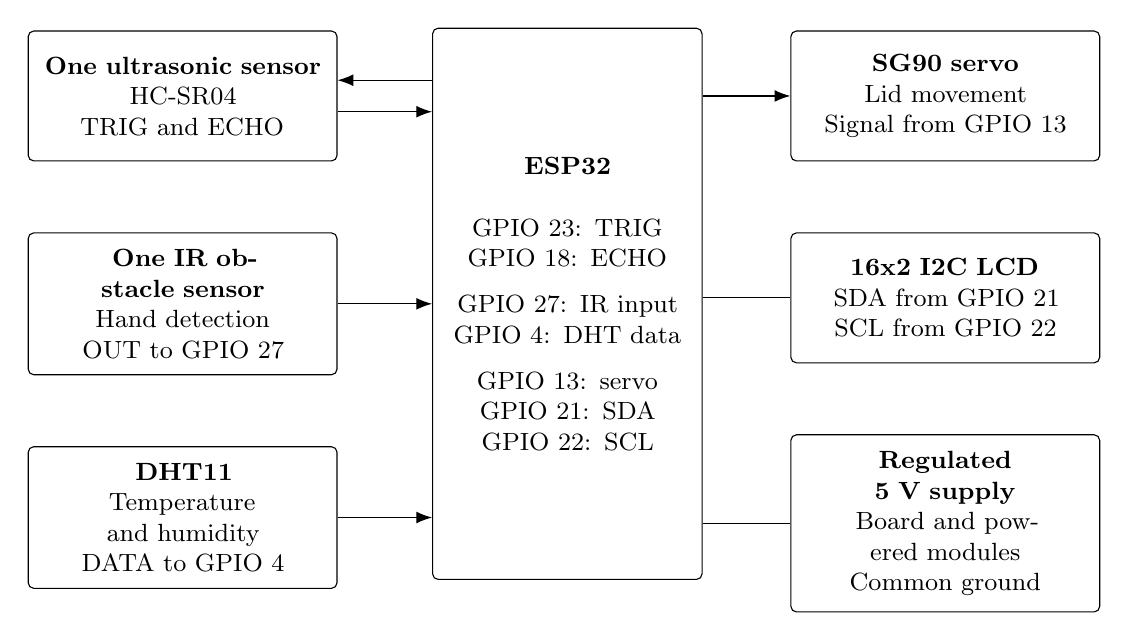
\begin{tikzpicture}[
  component/.style={draw,rounded corners=2pt,align=center,
    font=\small,text width=3.5cm,minimum height=1.65cm,
    inner sep=6pt,execute at begin node={\setlength{\parskip}{0pt}}},
  controller/.style={component,text width=3.0cm,minimum height=7.0cm},
  node distance=9mm]
% Nodes in each column are placed below the previous node's actual edge.
% Text wrapping can therefore increase a box height without overlap.
\node[component] (ultra) at (0,0)
  {\textbf{One ultrasonic sensor}\\HC-SR04\\TRIG and ECHO};
\node[component,below=of ultra] (ir)
  {\textbf{One IR obstacle sensor}\\Hand detection\\OUT to GPIO 27};
\node[component,below=of ir] (dht)
  {\textbf{DHT11}\\Temperature and humidity\\DATA to GPIO 4};
\node[controller,right=12mm of ir] (esp)
  {\textbf{ESP32}\\[4mm]
   GPIO 23: TRIG\\GPIO 18: ECHO\\[2mm]
   GPIO 27: IR input\\GPIO 4: DHT data\\[2mm]
   GPIO 13: servo\\GPIO 21: SDA\\GPIO 22: SCL};
\node[component] (servo) at ([xshift=4.8cm]esp.center |- ultra.center)
  {\textbf{SG90 servo}\\Lid movement\\Signal from GPIO 13};
\node[component,below=of servo] (lcd)
  {\textbf{16x2 I2C LCD}\\SDA from GPIO 21\\SCL from GPIO 22};
\node[component,below=of lcd] (power)
  {\textbf{Regulated 5 V supply}\\Board and powered modules\\Common ground};
\draw[arrow] ([yshift=2mm]esp.west |- ultra.east)
  -- ([yshift=2mm]ultra.east);
\draw[arrow] ([yshift=-2mm]ultra.east)
  -- ([yshift=-2mm]esp.west |- ultra.east);
\draw[arrow] (ir.east) -- (esp.west |- ir.east);
\draw[arrow] (dht.east) -- (esp.west |- dht.east);
\draw[arrow] (esp.east |- servo.west) -- (servo.west);
\draw[wire] (esp.east |- lcd.west) -- (lcd.west);
\draw[wire] (power.west) -- (esp.east |- power.west);
\end{tikzpicture}
\end{center}
\textbf{Figure 5.1} Proposed component connections for the physical bin.\par

The arrows show sensor and control signals. All components share a common ground. The ultrasonic input and LCD connection use suitable voltage matching, as required by the selected modules.\par

\textbf{Table 5.1 Sensor and control connections}\par
\begin{tabularx}{\textwidth}{@{}lY@{}}
\toprule
\textbf{Component signal} & \textbf{ESP32 connection} \\ \midrule
Ultrasonic TRIG & GPIO 23 \\
Ultrasonic ECHO & GPIO 18 through voltage matching \\
IR sensor OUT & GPIO 27 \\
DHT11 DATA & GPIO 4 \\
Servo control & GPIO 13 \\
LCD SDA and SCL & GPIO 21 and GPIO 22 through suitable I2C voltage matching \\
\bottomrule
\end{tabularx}

\clearpage
\reportsubsection{5.2 Working Principle}
\subsection*{System architecture}
The controller handles the lid and reads the sensors at the bin. It sends readings over the same local Wi-Fi network used by the collector's browser. The server checks those readings, stores them, and prepares the information shown on the dashboard.\par

\begin{center}
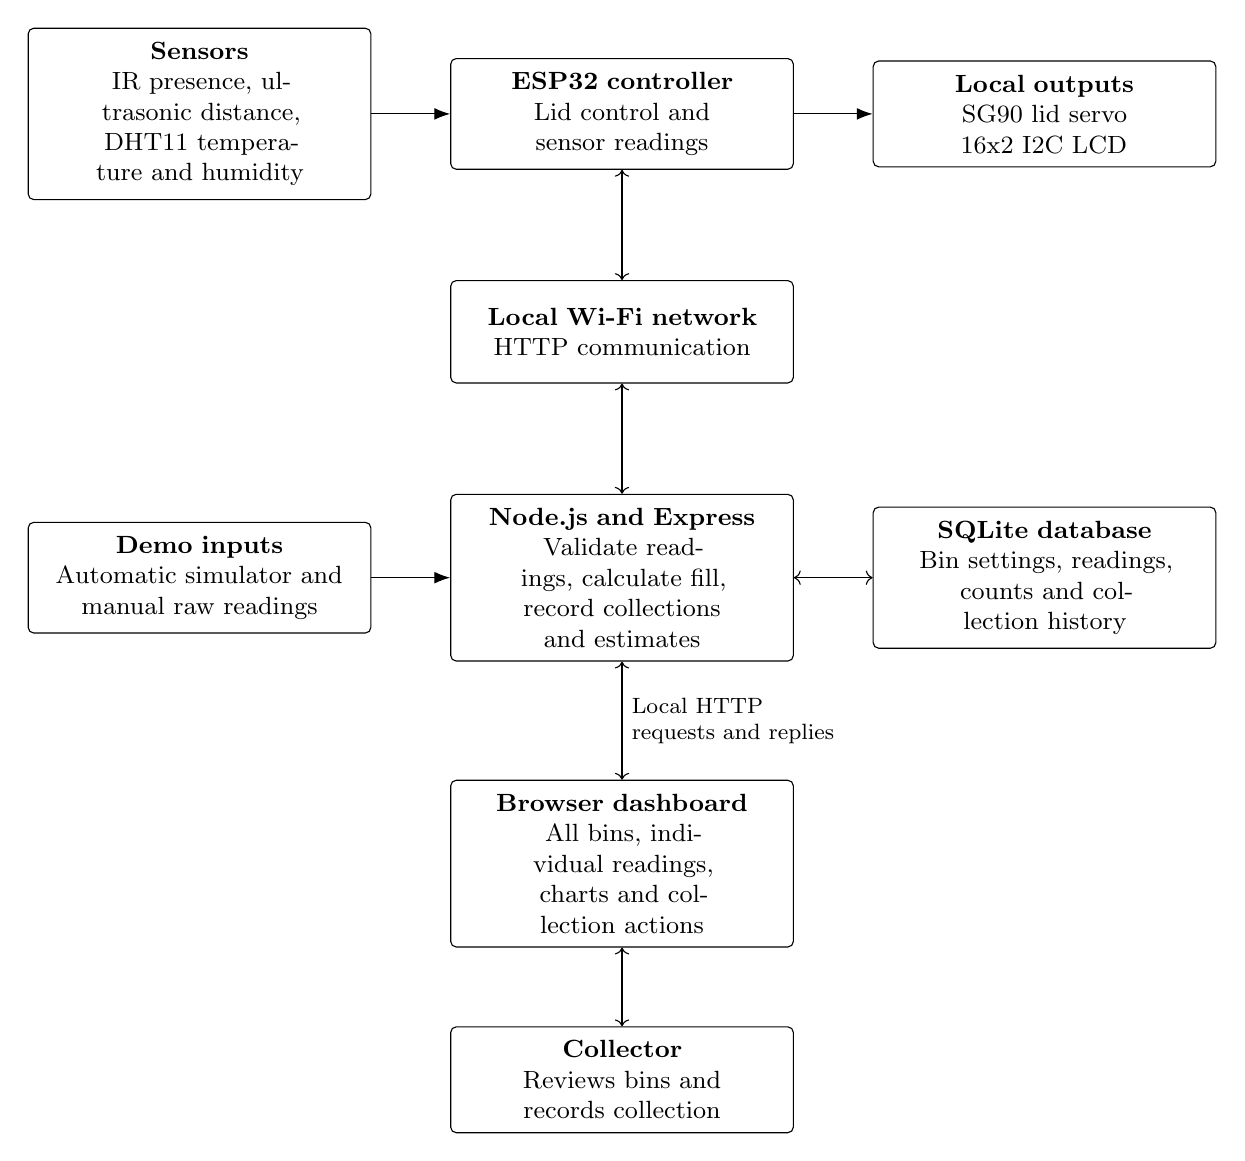
\begin{tikzpicture}[node distance=10mm and 10mm,
block/.append style={text width=4.0cm,minimum height=13mm}]
\node[block] (esp) {\textbf{ESP32 controller}\\Lid control and sensor readings};
\node[block,left=of esp] (sensors) {\textbf{Sensors}\\IR presence, ultrasonic distance,\\DHT11 temperature and humidity};
\node[block,right=of esp] (outputs) {\textbf{Local outputs}\\SG90 lid servo\\16x2 I2C LCD};
\node[block,below=14mm of esp] (wifi) {\textbf{Local Wi-Fi network}\\HTTP communication};
\node[block,below=14mm of wifi] (server) {\textbf{Node.js and Express}\\Validate readings, calculate fill,\\record collections and estimates};
\node[block,left=of server] (demo) {\textbf{Demo inputs}\\Automatic simulator and\\manual raw readings};
\node[block,right=of server] (db) {\textbf{SQLite database}\\Bin settings, readings,\\counts and collection history};
\node[block,below=15mm of server] (web) {\textbf{Browser dashboard}\\All bins, individual readings,\\charts and collection actions};
\node[block,below=10mm of web] (collector) {\textbf{Collector}\\Reviews bins and records collection};
\draw[arrow] (sensors) -- (esp);
\draw[arrow] (esp) -- (outputs);
\draw[arrow,<->] (esp) -- (wifi);
\draw[arrow,<->] (wifi) -- (server);
\draw[arrow] (demo) -- (server);
\draw[arrow,<->] (server) -- (db);
\draw[arrow,<->] (server) -- node[right,font=\footnotesize,align=left]{Local HTTP\\requests and replies} (web);
\draw[arrow,<->] (web) -- (collector);
\end{tikzpicture}
\end{center}
\textbf{Figure 5.2} System architecture of the proposed local Smart Dustbin.\par

Both demo input methods use the same reading API as the physical bin. For the current software demonstration, the demo inputs supply the readings without connecting hardware. The browser and server communicate locally; no cloud service is required.\par

\clearpage
\section*{5.2 Working Principle Continued}
\subsection*{Reading and sending data}
The proposed lid clear delay is 3 seconds, followed by a 2 second cooldown; hand detection during closing requests reopening. Distance sampling starts 2 seconds after the lid closes and uses the median of five usable samples. Readings are sent every 5 to 10 seconds without blocking local lid control. Startup does not count as an opening.\par


\subsection*{Turning distance into fill}
The empty distance E is measured from the sensor to the empty bin floor. The full distance F is measured to the highest permitted waste level. For a usable reading d, the server calculates:\newline \textbf{Fill percentage = 100 \(\times\) (E minus d) / (E minus F)}\newline The result is limited to 0 through 100. Calibration must satisfy E > F > 0. For example, E = 40 cm, F = 5 cm, and d = 19 cm gives 60\% fill.\par

\subsection*{Recognizing a collection}
A single low reading may be noise. The server therefore waits for three readings whose spread is no more than 5 percentage points and takes their median. If the previous stable fill was at least 70\% and the new stable fill is at most 10\%, it records a collection. It will not keep recording collections while the bin stays empty.\par

The manual button covers an emptying that does not meet this rule. After confirmation, it records the event and waits for fresh stable fill to set the new starting level. Earlier stable readings are cleared so they do not trigger another collection for the same emptying; the action does not create an assumed zero fill reading.\par

\subsection*{Estimating the next visit}
After collection, the server divides the rise in stable fill by the elapsed hours. With at least five stable points spanning ten minutes since collection and a positive rate, it divides the remaining fill to the target by that rate. The result is an estimate, not a promise. The dashboard shows ``Collect now'' at 90\%, or explains when data is missing, too old, or insufficient.\par


\clearpage
\reportsubsection{5.3 Flowchart}
The controller repeats its local checks while the system is running. Network work is scheduled separately so a slow request does not stop the lid from responding. Start and End below mark the demonstration session, rather than each sensor reading.\par

\begin{center}
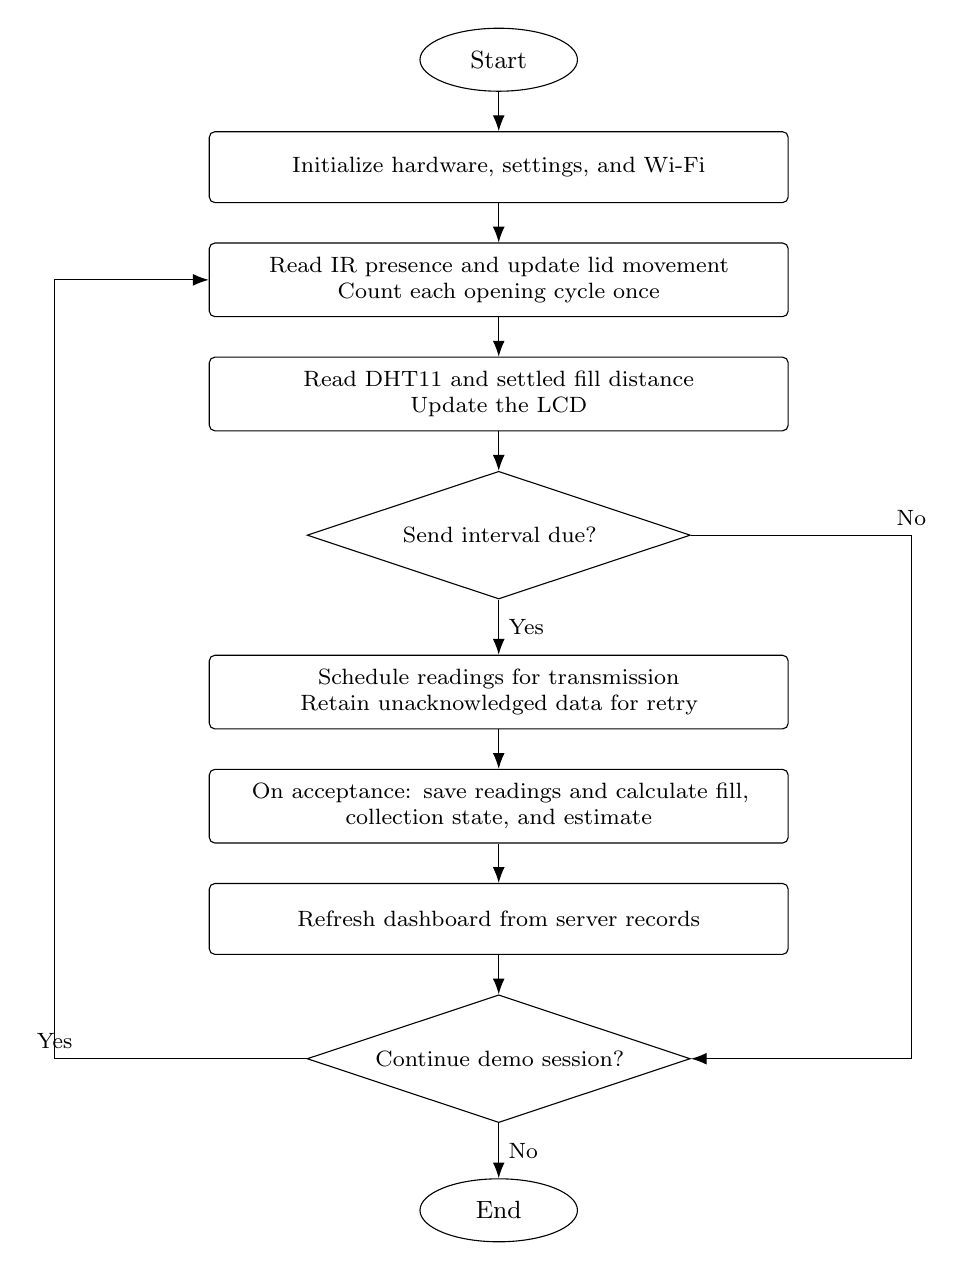
\begin{tikzpicture}[node distance=5mm,
block/.append style={text width=7.0cm,minimum height=9mm,font=\footnotesize},
terminal/.style={draw,ellipse,minimum width=2cm,minimum height=8mm,font=\small},
decision/.style={draw,diamond,aspect=3,align=center,inner sep=1pt,text width=4cm,font=\footnotesize}]
\node[terminal] (start) {Start};
\node[block,below=of start] (init) {Initialize hardware, settings, and Wi-Fi};
\node[block,below=of init] (local) {Read IR presence and update lid movement\\Count each opening cycle once};
\node[block,below=of local] (sample) {Read DHT11 and settled fill distance\\Update the LCD};
\node[decision,below=of sample] (due) {Send interval due?};
\node[block,below=7mm of due] (send) {Schedule readings for transmission\\Retain unacknowledged data for retry};
\node[block,below=of send] (server) {On acceptance: save readings and calculate fill,\\collection state, and estimate};
\node[block,below=of server] (view) {Refresh dashboard from server records};
\node[decision,below=of view] (run) {Continue demo session?};
\node[terminal,below=7mm of run] (end) {End};
\foreach \a/\b in {start/init,init/local,local/sample,sample/due,send/server,server/view,view/run}{\draw[arrow] (\a) -- (\b);}
\draw[arrow] (due) -- node[right,font=\footnotesize]{Yes} (send);
\draw[arrow] (due.east) -- ++(28mm,0) node[above,font=\footnotesize]{No} |- (run.east);
\draw[arrow] (run.west) -- ++(-32mm,0) node[above,font=\footnotesize]{Yes} |- (local.west);
\draw[arrow] (run) -- node[right,font=\footnotesize]{No} (end);
\end{tikzpicture}
\end{center}
\textbf{Figure 5.3} Main flow with separate Start and End symbols.\par

The server and browser steps occur independently of the controller loop. If a request fails, the controller keeps running and retries later; End means that the operator has stopped the demonstration.\par

\clearpage

\reportsection{6 System Interaction Model}
\reportsubsection{6.1 Use case diagram}
This model focuses on one collector task: recording a collection after emptying a bin when automatic detection has not recorded it.\par

\begin{center}
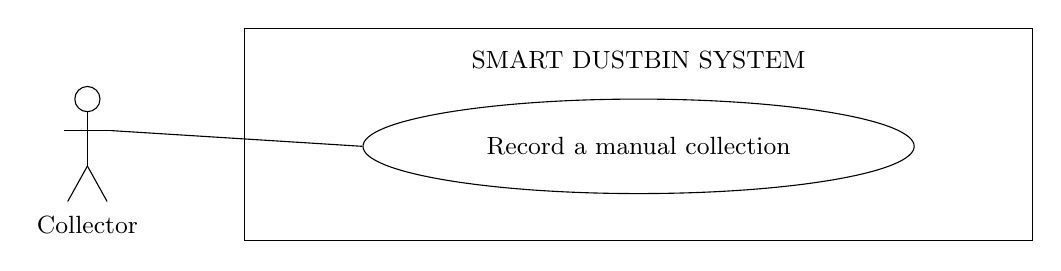
\begin{tikzpicture}[font=\small]
\draw (2,0) rectangle (12,2.7);
\node at (7,2.3) {SMART DUSTBIN SYSTEM};
\draw (0,1.8) circle (0.16);
\draw (0,1.64) -- (0,0.95);
\draw (-0.3,1.4) -- (0.3,1.4);
\draw (0,0.95) -- (-0.25,0.5);
\draw (0,0.95) -- (0.25,0.5);
\node at (0,0.2) {Collector};
\node[ellipse,draw,minimum width=7cm,minimum height=12mm] (collect) at (7,1.2) {Record a manual collection};
\draw (0.3,1.4) -- (collect.west);
\end{tikzpicture}
\end{center}
\textbf{Figure 6.1} Use case UC01: Record a manual collection.\par

\reportsubsection{6.2 Use case specification: UC01}
\begin{tabularx}{\textwidth}{@{}lY@{}}
\toprule
\textbf{Field} & \textbf{Description} \\ \midrule
Primary actor & Collector \\
Goal & Record that the selected bin has been emptied. \\
Preconditions & The bin is registered, the collector has emptied it, and its detail page is open. \\
Trigger & The collector selects ``Mark as collected.'' \\
\bottomrule
\end{tabularx}

\subsection*{Main flow}
1. The dashboard asks the collector to confirm the selected bin's name.\par
2. The collector confirms the collection.\par
3. The dashboard submits the request and disables repeat submission while saving.\par
4. The server saves one manual collection event with its time and resets the opening count.\par
5. The dashboard shows the updated collection time, count, and history.\par

\subsection*{Alternative flows}
\textbf{Cancellation:} If the collector cancels at step 2, the dialog closes without changing the bin record.\par
\textbf{Save failure:} If the server cannot confirm the save, the dashboard shows an error and allows a retry using the same request ID to avoid duplicate records.\par
\textbf{Offline bin:} A manual collection can still be recorded when the server is available, but fill remains last known until a fresh reading arrives.\par

\subsection*{Postconditions}
On success, one manual event is stored and the opening count is zero. The earlier detection window is cleared, and fresh stable readings establish the next fill baseline without inventing an empty reading. Cancellation leaves the record unchanged.\par

\clearpage

\reportsection{7 Limitations and Future Scope}
\reportsubsection{7.1 What the prototype cannot prove}
The demonstration will use one real bin. Simulated bins will help show how the dashboard handles several records, but they cannot prove that many physical bins would perform equally well outside the laboratory.\par

Fill sensing also has limits. A level surface reflects sound differently from a loose pile of paper or an angled object. The measured percentage describes relative fill height, which may differ from the actual volume of waste. Calibration and repeated samples can help, but they cannot remove every error.\par

Opening counts are another estimate of activity. A person may open the lid without dropping anything, or place several items inside during one opening. Pending counts may also be lost if the ESP32 loses power before sending them. There is no separate sensor to confirm that the lid physically reached its intended position.\par

Automatic collection detection works only for the specified change in stable fill. It may miss partial emptying, early collection, or a gradual drop through several intermediate levels. The manual collection button covers these cases, but it relies on the collector entering the event correctly.\par

The next collection estimate assumes that recent filling continues at a similar rate. Real use can change during the day. A fast demonstration may also produce an estimate of only a few minutes. The system will label this as an estimate and avoid displaying one when there is too little reliable data.\par

The DHT11 provides supporting information, not a certified heat or fire warning. The circuit is not designed for exposure to water or heavy waste. The lid has no dedicated obstruction sensor. Finally, the local dashboard depends on a running computer and a trusted Wi-Fi network.\par

\reportsubsection{7.2 How the project could grow}
The first useful step would be to test more physical bins for a longer period. This would show how often fill readings drift and how well the collection rules work with real waste. The findings could guide better sensors, revised mounting, and more suitable thresholds.\par

Later versions could preserve counts across power failures, add lid position or obstruction sensing, and improve the enclosure. User accounts, encrypted communication, and backups would be needed before wider use. Maps, routes, and remote access could then be considered as separate additions.\par


\clearpage
\reportsection{8 Appendix}
\reportsubsection{8.1 References}

[R1] Group 06. Smart Dustbin Project Proposal Corrected. Computer Interfacing Laboratory, Bangladesh University of Professionals. Submitted 21 September 2026. Supplied project proposal.\par

[R2] Smart Dustbin: Collector Dashboard, Planning Document. Supplied planning text. Includes confirmed choices, suggested settings, and open decisions.\par

[R3] System Requirements Specification Report Guideline. Supplied course guideline. Defines the report structure and page limit.\par

[R4] Arduino Education. Trash Can Project. \href{https://www.arduino.cc/education/smart-trash-can}{Arduino Education project page}. Accessed 4 October 2026.\par

[R5] Arduino Cloud. Smart Trash Can. \href{https://cloud.arduino.cc/use-cases-home-automation-smart-trash-can/}{Arduino Cloud project page}. Accessed 4 October 2026.\par

[R6] Espressif Systems. ESP32 Series Datasheet. \href{https://documentation.espressif.com/esp32_datasheet_en.html}{Official ESP32 datasheet}. Accessed 4 October 2026. Check the selected development board separately.\par


[R7] NASA. Appendix C: How to Write a Good Requirement. \href{https://www.nasa.gov/reference/appendix-c-how-to-write-a-good-requirement/}{NASA requirements guidance}. Accessed 10 October 2026.\par

[R8] IBM. What is requirements management? \href{https://www.ibm.com/think/topics/what-is-requirements-management}{Functional and nonfunctional requirements overview}. Accessed 10 October 2026.\par

\end{document}
